\setcounter{ex}{0} %Âu Lạc
\subsection{Trắc nghiệm (2 điểm)}
\Opensolutionfile{ans}[ans/ans6]
%%Câu 1:
\begin{ex}
Biểu thức $\sqrt{2x-6}$ có điều kiện xác định là
\choice
{$x<3$}
{\True $x\ge 3$}
{$x\le 3$}
{$x>3$}
\end{ex}

%%Câu 2:
\begin{ex}
Điều kiện xác định của phương trình $\dfrac{4x-1}{x}+1=\dfrac{3}{x+2}$ là
\choice
{$x\neq -2$}
{$x\neq 2$}
{$x\neq 0$}
{\True $x\neq 0,\,x\neq -2$}
\end{ex}

%%Câu 3:
\begin{ex}
Chọn câu đúng. Trong một đường tròn, số đo cung nhỏ bằng:
\choice
{Số đo cung lớn}
{\True Số đo của góc ở tâm chắn cung đó}
{Số đo của góc ở tâm chắn cung lớn}
{Số đo của cung nửa đường tròn}
\end{ex}

%%Câu 4:
\begin{ex}
Nếu $a<b$ thì $2a+3 \square 2b+3$ bằng:
\choice
{$\ge$}
{$\le$}
{\True $<$}
{$>$}
\end{ex}

%%Câu 5:
\begin{ex}
Bất phương trình $2-3x\ge 5$ có nghiệm là:
\choice
{$x\ge -1$}
{$x\le1$}
{$x\ge 1$}
{\True $x\le -1$}
\end{ex}

%%Câu 6:
\begin{ex}
Rút gọn $\sqrt{\dfrac{(a-4)^2}{4}}$ với $a<4$ ta được:
\choice
{\True $\dfrac{4-a}{2}$}
{$\dfrac{a+4}{4}$}
{$\dfrac{a-4}{2}$}
{$\dfrac{4-a}{4}$}
\end{ex}

%%Câu 7:
\begin{ex}
Kết quả của phép tính $3\sqrt{(-2)^2}+(\sqrt{2})^2-2\sqrt{3^2}$ là:
\choice
{$-2$}
{\True $2$}
{$10$}
{$-10$}
\end{ex}

%%Câu 8:
\begin{ex}
Cho hai đường tròn $(O;5\,\text{cm})$ và $(O';4\,\text{cm})$ với $OO'=1\,\text{cm}$. Kết luận nào sau đây \textbf{đúng} về vị trí tương đối của hai đường tròn?
\choice
{Hai đường tròn cắt nhau}
{Hai đường tròn ở ngoài nhau}
{Hai đường tròn tiếp xúc ngoài}
{\True Hai đường tròn tiếp xúc trong}
\end{ex}

%%Câu 9:
\begin{ex}
Tìm giá trị của $m$ để hệ phương trình 
$\begin{cases} 
2x-y=4\\ 
(m-1)x+2y=m 
\end{cases}$ vô nghiệm:
\choice
{$m\ne-3$}
{$m>-3$}
{\True $m=-3$}
{$m<-3$}
\end{ex}

%%Câu 10:
\begin{ex}
Cho biết $\tan \alpha=\dfrac{2}{3}$. Tính giá trị biểu thức: $\dfrac{\sin^3 x+3\cos^3 x}{27\sin^3 x-25\cos^3 x}$
\choice
{$\dfrac{89}{891}$}
{$\dfrac{89}{159}$}
{\True $\dfrac{-89}{459}$}
{$\dfrac{89}{459}$}
\end{ex}

\Closesolutionfile{ans}
\Opensolutionfile{ansbook}[ans/ansbook6]

\setcounter{bt}{0}
\subsection{Tự luận (8 điểm)}

%%Bài 1:
\begin{bt}[1 điểm]
Giải phương trình, hệ phương trình sau:
\begin{listEX}[2]
\item $(6-2x)(3x+6)=0$
\item $\begin{cases}
2x+3y=-16\\
2x-2y=-1
\end{cases}$
\end{listEX}
\loigiai{
a) $x=3,x=-2$ \hspace{2cm} b) $\left(\dfrac{-7}{2};-3\right)$
}
\end{bt}

%%Bài 2:
\begin{bt}[1 điểm]
Rút gọn các biểu thức sau:
\begin{listEX}[2]
\item $\sqrt{11-6\sqrt{2}}+\sqrt{11+6\sqrt{2}}$
\item $\dfrac{26}{4-\sqrt{3}}+\dfrac{3-\sqrt{6}}{\sqrt{3}-\sqrt{2}}$
\end{listEX}
\loigiai{
a) 6 \hspace{2cm} b) $8+3\sqrt{3}$
}
\end{bt}

%%Bài 3:
\begin{bt}[1 điểm]
Điện áp $V$ (tính theo Volt) yêu cầu cho một mạch điện được cho bởi công thức $V=\sqrt{PR}$, trong đó $P$ là công suất (tính theo Watt) và $R$ là điện trở (tính theo Ohm).  
\begin{enumerate}
\item Cần điện áp bao nhiêu Volt để thắp sáng một bóng đèn A có công suất $100$ Watt và điện trở $110$ Ohm? \textit{(kết quả làm tròn đến hàng đơn vị)}
\item Bóng đèn B có điện áp bằng $110$ Volt, điện trở trong là $88$ Ohm có công suất lớn hơn bóng đèn A không? Vì sao?
\end{enumerate}
\loigiai{
a) $V\approx 105$ (volt) \hspace{2cm} b) $P=\dfrac{275}{2}>100$
}
\end{bt}

%%Bài 4:
\begin{bt}[1 điểm]
Trường THCS Âu Lạc tổ chức cho học sinh khối 8 và khối 9 đi tham quan tại khu di tích lịch sử Rạch Gầm - Xoài Mút cho 363 người gồm học sinh và giáo viên phụ trách, nhà trường đã thuê 10 chiếc xe du lịch gồm 2 loại: Loại 45 chỗ ngồi và loại 16 chỗ ngồi (không kể tài xế). Hỏi nhà trường cần thuê bao nhiêu chiếc xe mỗi loại? Biết rằng không có xe nào còn chỗ trống.
\loigiai{
Nhà trường thuê 7 xe 45 chỗ và 3 xe 16 chỗ.
}
\end{bt}

%%Bài 5:
\begin{bt}[1 điểm]
\immini[thm]
{Bánh xe (khi bơm căng) của một chiếc xe đạp có đường kính $650\,\text{mm}$.  
Biết rằng khi giò đĩa quay một vòng thì bánh xe đạp quay được 3 vòng. (hình vẽ)
\begin{enumerate}
\item Tính chu vi của bánh xe đạp (khi bơm căng).
\item Hỏi chiếc xe đạp di chuyển được quãng đường dài bao nhiêu mét khi giò đĩa quay 10 vòng liên tục?\\
\textit{Câu a, b kết quả làm tròn đến hàng đơn vị}
\end{enumerate}
}
{
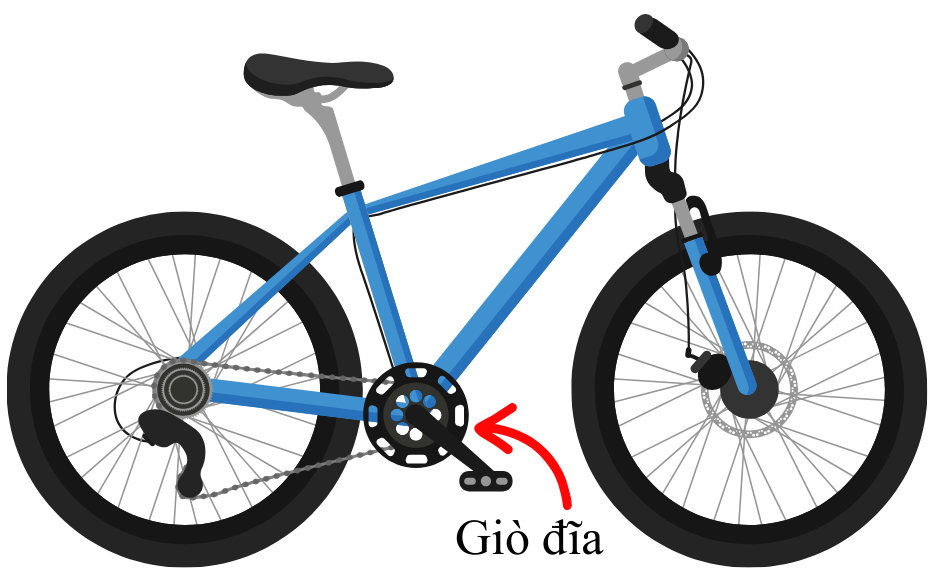
\includegraphics[height=4cm]{hinh/De6-1.png}
}
\loigiai{
a) $C\approx 2024$ (mm) \hspace{2cm} b) $10\cdot 3\cdot 650\pi=19500\pi\,(\text{mm})\approx61\,(\text{m})$
}
\end{bt}

%%Bài 6:
\begin{bt}[3,0 điểm]
Cho đường tròn $(O;R)$ đường kính $AB$. Kẻ tiếp tuyến $Ax$, lấy $P$ trên $Ax$ ($AP>R$). Từ $P$ kẻ tiếp tuyến $PM$ với $(O)$ ($M$ là tiếp điểm). 
\begin{enumerate}
    \item Chứng minh rằng bốn điểm $A, P, M, O$ cùng thuộc một đường tròn và $BM \parallel OP$.
    \item Đường thẳng vuông góc với $AB$ tại $O$ cắt tia $BM$ tại $N$. Chứng minh tứ giác $OBNP$ là hình bình hành.
    \item Giả sử $AN$ cắt $OP$ tại $K$; $PM$ cắt $ON$ tại $I$; $PN$ cắt $OM$ tại $J$. Chứng minh $I, J, K$ thẳng hàng.
\end{enumerate}
\loigiai{ 
\immini{
\begin{enumerate}
    \item $A,P,O,M$ cùng nằm trên đường tròn đường kính $OP$
    
    Ta có $OP\perp AM, BM\perp AM$ suy ra $OP\parallel BM$.
    \item $\triangle AOP = \triangle OBN \Rightarrow OP = BN$
    
    Ta lại có $BN \parallel OP$ nên $OBNP$ là hình bình hành.

    \item Chứng minh  $I$ là trực tâm $\triangle POJ$ suy ra $IJ \perp OP$ (1)

    Chứng minh $K$ là trung điểm $OP$.

    Lại có: $\widehat{APO} = \widehat{OPI} = \widehat{IOP}$
    
    Suy ra $\triangle IPO$ cân tại $I$ suy ra $IK \perp OP$ (2)

    Từ (1) và (2) suy ra $I, J, K$ thẳng hàng.
\end{enumerate}
}
{
	\begin{tikzpicture}[scale=1, font=\footnotesize, line join =round, line cap=round, >=stealth]
		\def\r{1.8}
		\path 
		(0,0) coordinate (O)
		(180:\r) coordinate (A)
		(0:\r) coordinate (B)
		(-\r,2.5*\r) coordinate (x)node[left]{$x$}
		($(A)!4/5!(x)$) coordinate (P)
		($(O)!(A)!(P)$) coordinate (H)
		($(A)!2!(H)$) coordinate (M)
		($(O)!1cm!-90:(A)$) coordinate (n')
		(intersection of B--M and O--n') coordinate (N)
		(intersection of A--N and O--P) coordinate (K)
		(intersection of O--N and M--P) coordinate (I)
		(intersection of O--M and N--P) coordinate (J)
		;
		\draw 
		(O) circle (\r) 
		(x)--(A)--(B)--(N)--(A)--(M)--(P)--(O)--(N) (P)--(J)--(O)
		;
		\draw[dashed] (K)--(J);
		\foreach \x/\g in{O/-90,A/180,B/0,P/180,K/160,M/0,N/90,I/120,J/40}
		\draw[fill=white] (\x) circle (1.5pt) +(\g:.3) node{$\x$};
	\end{tikzpicture}
}
}
\end{bt}
\Closesolutionfile{ansbook}